\documentclass{report}
\usepackage[utf8]{inputenc}

% Títulos automáticos en español
\usepackage[english]{babel}

% Soporte para buenas urls e hipervínculos entre secciones
\usepackage{hyperref}

% Imágenes y figuras
\usepackage{graphicx}

\usepackage{tikz}
\usetikzlibrary{automata, positioning, arrows.meta}

\def \unidad{Computer Engineering Department}
\def \programa{Computer Engineering}
\def \curso{IC5701 - Compilers \& Interpreters}
\def \subtitulo {Dr. Francisco J. Torres-Rojas}
\def \titulo{Deterministic Finite Automatons}
\def \autores{
    Javier Lee Liang\\
    2020184824\\
    
    \vspace{0.5cm}
    
    Steven D. Loaíciga Segura\\
    2024214083

    \vspace{0.5cm}
    
    Luan Valverde Villalobos\\
    2024080542
}
\def \fecha{October 2026}
\def \lugar{
    San Jose, 
    Costa Rica
}

% Inicia el documento 
\begin{document}

\begin{titlepage}
    \begin{center}
        \vspace*{1cm}
        
        \includegraphics[width=0.8\linewidth]{figures/logo_tec.jpg}\\
        \LARGE
        \unidad\\
        \programa\\
        \curso
        
        \vspace{1cm}
        
        \Huge
        \textbf{\titulo}
            
        \vspace{0.5cm}
        \LARGE
        \subtitulo
            
        \vspace{1.5cm}
        
        \large    
        \autores
            
        \vfill
        
        \lugar\\
        \fecha
        
    \end{center}
\end{titlepage}

\chapter*{Exercises to solve}

\section*{Page of the exercises}

\begin{figure}[h]
    \centering
    \includegraphics[width=0.8\linewidth]{figures/exercises.png}
    \caption{Exercises to solve. Starting from the number 12 to 36}
\end{figure}

\chapter*{Exercises solved}

\section*{Exercise 12}
The set of strings over \{\textit{a,b,c}\} in which all the \textit{a}'s precede the \textit{b}'s, which in turn precede the \textit{c}'s. It is possible that there are no \textit{a}'s, \textit{b}'s, or \textit{c}'s.

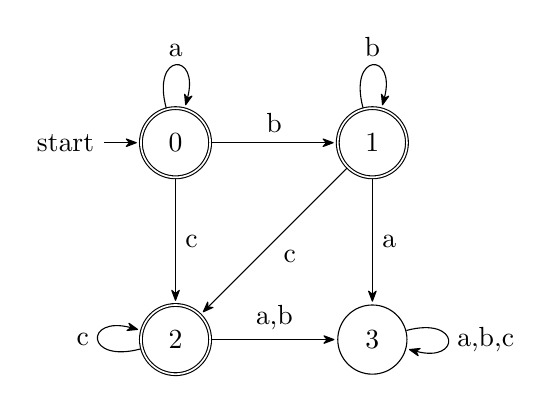
\begin{tikzpicture}[
    shorten >=1pt, node distance=2.5cm, on grid, auto, >={Stealth[round]}
]
    % --- 1. DEFINE THE STATES ---
    \node[state, initial, accepting] (0) {$0$};
    \node[state, accepting] (1) [right=of 0] {$1$};
    \node[state, accepting] (2) [below=of 0] {$2$};
    \node[state] (3) [below=of 1] {$3$};

    % --- 2. DEFINE THE TRANSITIONS ---
    \path[->] 
        (0) edge [loop above] node {a} ()
            edge node {b} (1)
            edge node {c} (2)
        
        (1) edge [loop above] node {b} ()
            edge node {c} (2)
            edge node {a} (3)
        
        (2) edge [loop left] node {c} ()
            edge node {a,b} (3)

        (3) edge [loop right] node {a,b,c} ()
    
        ;
\end{tikzpicture}

\section*{Exercise 13}
The same set as Exercise 12 without the null string.

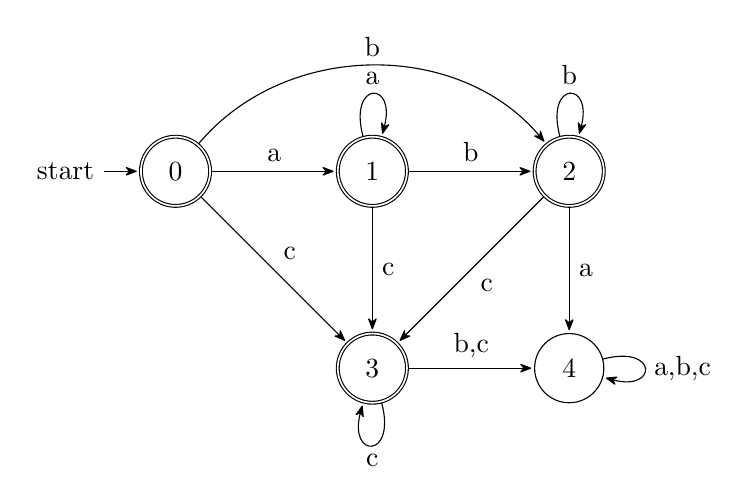
\begin{tikzpicture}[
    shorten >=1pt, node distance=2.5cm, on grid, auto, >={Stealth[round]}
]
    % --- 1. DEFINE THE STATES ---
    \node[state, initial, accepting] (0) {$0$};
    \node[state, accepting] (1) [right=of 0] {$1$};
    \node[state, accepting] (2) [right=of 1] {$2$};
    \node[state, accepting] (3) [below=of 1] {$3$};
    \node[state] (4) [below=of 2] {$4$};

    % --- 2. DEFINE THE TRANSITIONS ---
    \path[->] 
        (0) 
            edge node {a} (1)
            edge [bend left=50] node {b} (2)
            edge node {c} (3)
        
        (1) edge [loop above] node {a} ()
            edge node {b} (2)
            edge node {c} (3)
            
        (2) edge [loop above] node {b} ()
            edge node {a} (4)
            edge node {c} (3)

        (3) edge [loop below] node {c} ()
            edge node {b,c} (4)
        
        (4) edge [loop right] node {a,b,c} ()

        ;
\end{tikzpicture}

\section*{Exercise 14}
The set of strings of length two or more over \{\textit{a,b}\} in which all the \textit{a}'s precede the \textit{b}'s.

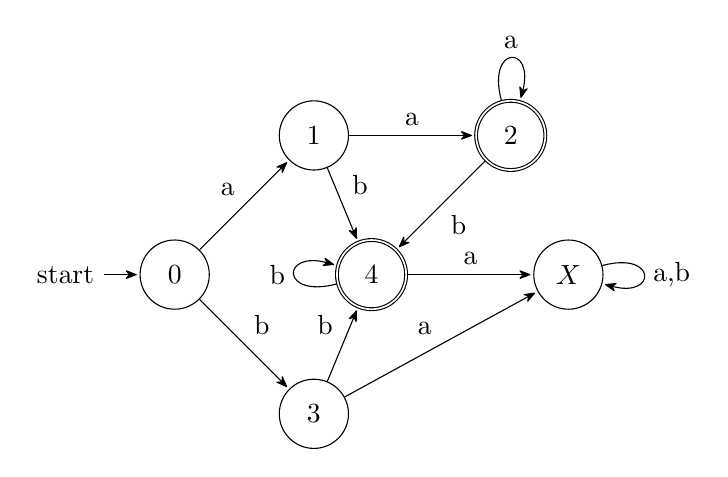
\begin{tikzpicture}[
    shorten >=1pt, node distance=2.5cm, on grid, auto, >={Stealth[round]}
]
    % --- 1. DEFINE THE STATES ---
    \node[state, initial] (0) {$0$};
    \node[state] (1) [above right=of 0] {$1$};
    \node[state, accepting] (2) [right=of 1] {$2$};

    \node[state] (3) [below right=of 0] {$3$};
    \node[state, accepting] (4) [right=of 0] {$4$};

    \node[state] (X) [right=of 4] {$X$};

\path[->] 
        (0) edge node {a} (1)
            edge node {b} (3)

        (1) edge node {a} (2)
            edge node {b} (4)

        (2) edge [loop above] node {a} ()
            edge node {b} (4)

        (3) edge node {a} (X)
            edge node {b} (4)

        (4) edge node {a} (X)
            edge [loop left] node {b} ()

        (X) edge [loop right] node {a,b} ()

        ;
    
\end{tikzpicture}

\section*{Exercise 15}
The set of strings over \{\textit{a,b}\} that contain the substring \textit{aa} and the substring \textit{bb}.

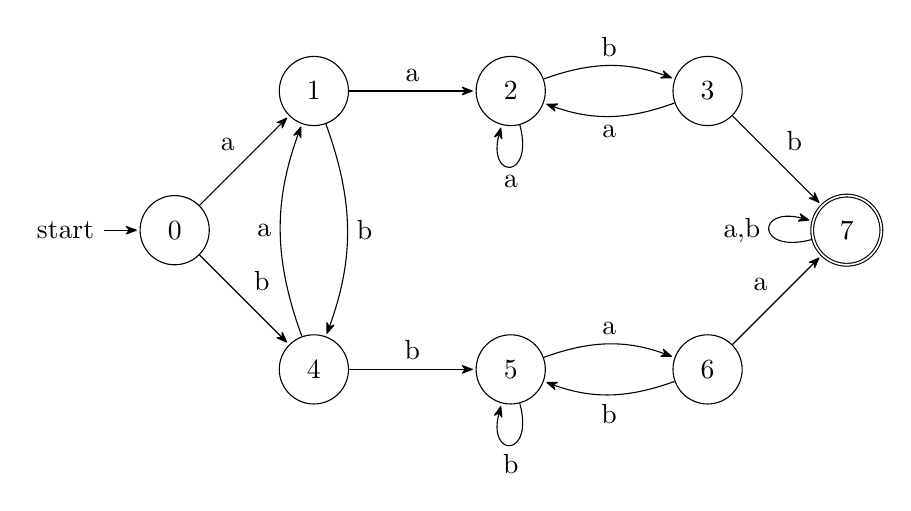
\begin{tikzpicture}[
    shorten >=1pt, node distance=2.5cm, on grid, auto, >={Stealth[round]}
]
    % --- 1. DEFINE THE STATES ---
    \node[state, initial] (0) {$0$};
    
    \node[state] (1) [above right=of 0] {$1$};
    \node[state] (2) [right=of 1] {$2$};
    \node[state] (3) [right=of 2] {$3$};
    
    \node[state] (4) [below right=of 0] {$4$};
    \node[state] (5) [right=of 4] {$5$};
    \node[state] (6) [right=of 5] {$6$};
    
    \node[state, accepting] (7) [below right=of 3] {$7$};

    \path[->] 
        (0) edge node {a} (1)
            edge node {b} (4)

        (1) edge node {a} (2)
            edge [bend left=20] node {b} (4)

        (2) edge [loop below] node {a} ()
            edge [bend left=20] node {b} (3)

        (3) edge [bend left=20] node {a} (2)
            edge node {b} (7)

        
        (4) edge [bend left=20] node {a} (1)
            edge node {b} (5)

        (5) edge [loop below] node {b} ()
            edge [bend left=20] node {a} (6)

        (6) edge node {a} (7)
            edge [bend left=20] node {b} (5)

        (7) edge [loop left] node {a,b} ()
        ; 

\end{tikzpicture}

\newpage

\section*{Exercise 16}
The set of strings over \{\textit{a,b}\} in which the substring \textit{aa} occurs at least twice. \textit{Hint}: Beware of the substring \textit{aaa}.

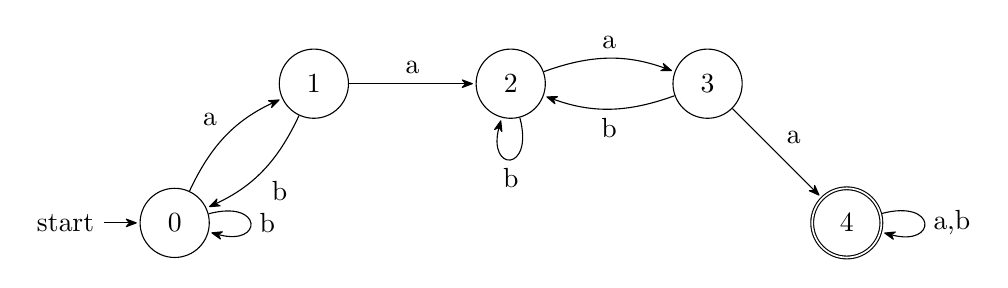
\begin{tikzpicture}[
    shorten >=1pt, node distance=2.5cm, on grid, auto, >={Stealth[round]}
]
    \node[state, initial] (0) {$0$};
    \node[state] (1) [above right=of 0] {$1$};
    \node[state] (2) [right=of 1] {$2$};
    \node[state] (3) [right=of 2] {$3$};
    \node[state, accepting] (4) [below right=of 3] {$4$};

    \path[->] 
        (0) edge [bend left=20] node {a} (1)
            edge [loop right] node {b} ()
        
        (1) edge node {a} (2)
            edge [bend left=20] node {b} (0)
            
        (2) edge [bend left=20] node {a} (3)
            edge [loop below] node {b} ()

        (3) edge node {a} (4)
            edge [bend left=20] node {b} (2)
        
        (4) edge [loop right] node {a,b} ()

        ;
\end{tikzpicture}


\section*{Exercise 17}
The set of strings over \{\textit{a,b,c}\} that do not contain the substring \textit{aa}.

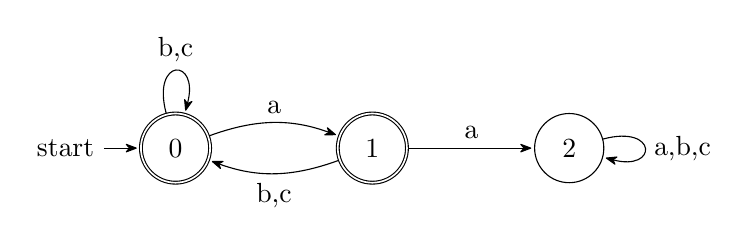
\begin{tikzpicture}[
    shorten >=1pt, node distance=2.5cm, on grid, auto, >={Stealth[round]}
]
    \node[state, initial, accepting] (0) {$0$};
    \node[state, accepting] (1) [right=of 0] {$1$};
    \node[state] (2) [right=of 1] {$2$};

    \path[->] 
        (0) edge [bend left=20] node {a} (1)
            edge [loop above] node {b,c} ()
        
        (1) edge node {a} (2)
            edge [bend left=20] node {b,c} (0)
            
        (2) edge [loop right] node {a,b,c} ()

        ;
\end{tikzpicture}

\section*{Exercise 18}
The set of strings over \{\textit{a,b}\} that do not begin with the substring \textit{aaa}.

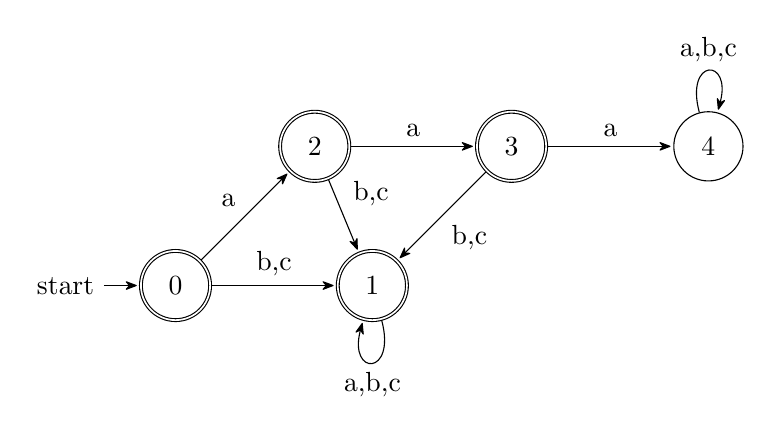
\begin{tikzpicture}[
    shorten >=1pt, node distance=2.5cm, on grid, auto, >={Stealth[round]}
]
    \node[state, initial, accepting] (0) {$0$};
    \node[state, accepting] (1) [right of=0] {$1$};

    \node[state, accepting] (2) [above right=of 0] {$2$};
    \node[state, accepting] (3) [right=of 2] {$3$};
    \node[state] (4) [right=of 3] {$4$};

    \path[->] 
        (0) edge node {a} (2)
            edge node {b,c} (1)
        
        (1) edge [loop below] node {a,b,c} ()
            
        (2) edge node {a} (3)
            edge node {b,c} (1)

        (3) edge node {a} (4)
            edge node {b,c} (1)
        
        (4) edge [loop above] node {a,b,c} ()

        ;
\end{tikzpicture}

\newpage

\section*{Exercise 19}
The set of strings over \{\textit{a,b}\} that do not contain with the substring \textit{aaa}.

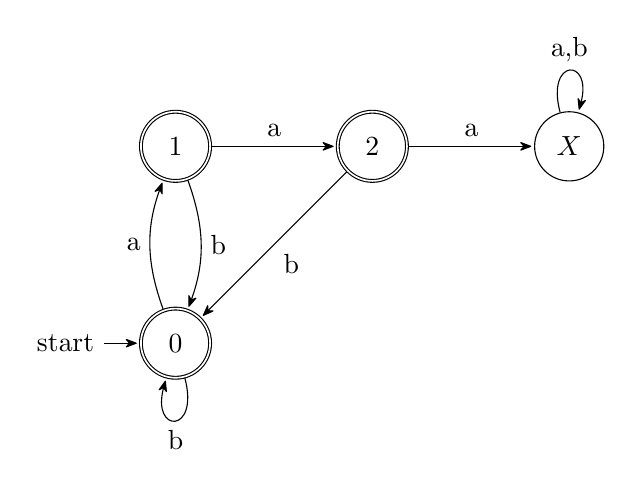
\begin{tikzpicture}[
    shorten >=1pt, node distance=2.5cm, on grid, auto, >={Stealth[round]}
]
    \node[state, initial, accepting] (0) {$0$};
    \node[state, accepting] (1) [above=of 0] {$1$};
    \node[state, accepting] (2) [right=of 1] {$2$};
    \node[state] (X) [right=of 2] {$X$};

    \path[->] 
        (0) edge [bend left=20] node {a} (1)
            edge [loop below] node {b} ()
        
        (1) edge node {a} (2)
            edge [bend left=20] node {b} (0)
            
        (2) edge node {a} (X)
            edge node {b} (0)
        
        (X) edge [loop above] node {a,b} ()

        ;
\end{tikzpicture}

\section*{Exercise 20}
The set of strings over \{\textit{a,b}\} that do not contain with the substring \textit{aba}.

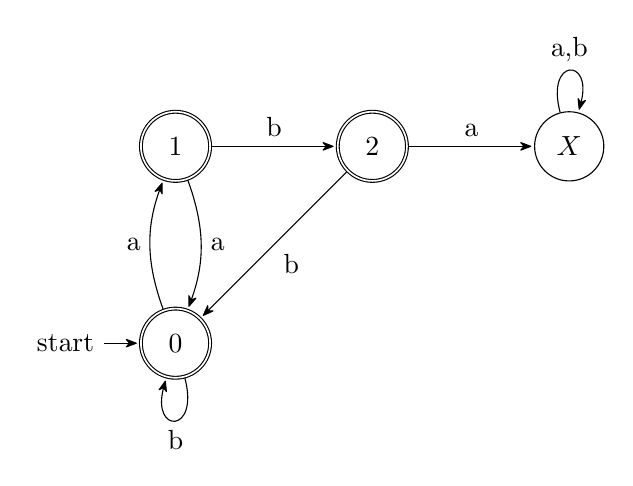
\begin{tikzpicture}[
    shorten >=1pt, node distance=2.5cm, on grid, auto, >={Stealth[round]}
]
    \node[state, initial, accepting] (0) {$0$};
    \node[state, accepting] (1) [above=of 0] {$1$};
    \node[state, accepting] (2) [right=of 1] {$2$};
    \node[state] (X) [right=of 2] {$X$};

    \path[->] 
        (0) edge [bend left=20] node {a} (1)
            edge [loop below] node {b} ()
        
        (1) edge node {b} (2)
            edge [bend left=20] node {a} (0)
            
        (2) edge node {a} (X)
            edge node {b} (0)
        
        (X) edge [loop above] node {a,b} ()

        ;
\end{tikzpicture}

\newpage

\section*{Exercise 21}
The set of strings over \{\textit{a,b}\} in which the substring \textit{aa} occurs extacly once.

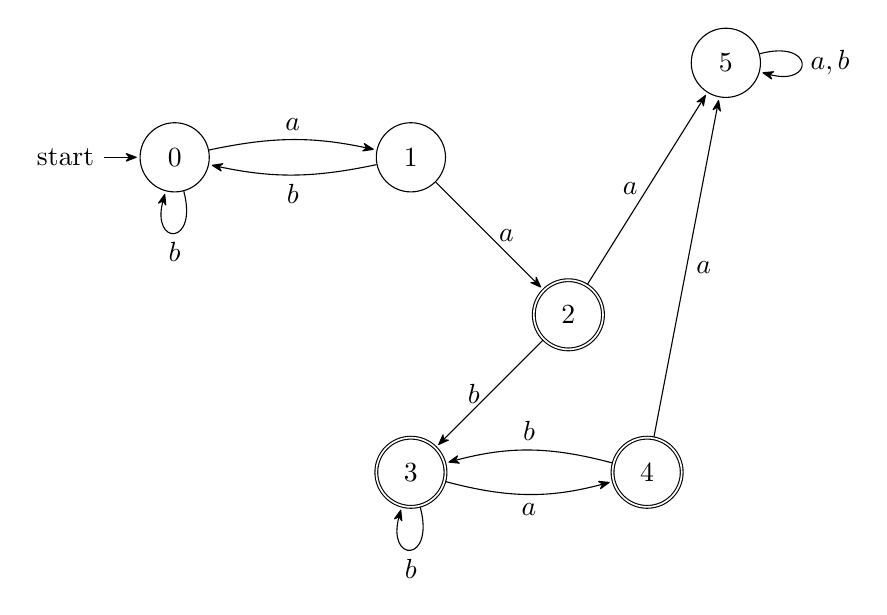
\begin{tikzpicture}[
    shorten >=1pt,          % Shortens arrows slightly so they don't touch node borders
    node distance=2.5cm,    % Sets global spacing between states
    on grid,                % Aligns positions based on center points instead of node borders
    auto,                   % Smart placement of transition labels
    >={Stealth[round]}      % Uses a clean, modern arrowhead style
]

% Estados
\node[state, initial, initial where=left] (0) at (0,0)    {0};
\node[state]                             (1) at (3,0)    {1};
\node[state, accepting]                  (2) at (5,-2)   {2};
\node[state, accepting]                  (3) at (3,-4)   {3};
\node[state, accepting]                  (4) at (6,-4)   {4};
\node[state]                             (5) at (7,1.2)  {5};

% Transiciones
\path[->]
    (0) edge[bend left=12] node[above] {$a$} (1)
    (0) edge[loop below]   node       {$b$} (0)

    (1) edge[bend left=12] node[below] {$b$} (0)
    (1) edge              node[right] {$a$} (2)

    (2) edge              node[left]  {$a$} (5)
    (2) edge              node[left]  {$b$} (3)

    (3) edge[bend right=15] node[below] {$a$} (4)
    (3) edge[loop below]    node        {$b$} (3)

    (4) edge[bend right=15] node[above] {$b$} (3)
    (4) edge               node[right] {$a$} (5)

    (5) edge[loop right]    node        {$a,b$} (5);
\end{tikzpicture}

\section*{Exercise 22}
The set of strings over \{\textit{a,b,c}\} that begin with \textit{a}, contain exactly two \textit{b}'s, and end with \textit{cc}.

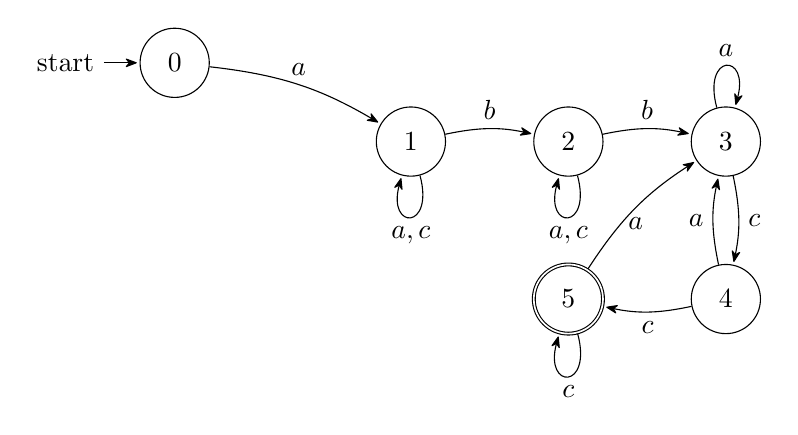
\begin{tikzpicture}[
    shorten >=1pt,          % Shortens arrows slightly so they don't touch node borders
    node distance=2.5cm,    % Sets global spacing between states
    on grid,                % Aligns positions based on center points instead of node borders
    auto,                   % Smart placement of transition labels
    >={Stealth[round]}      % Uses a clean, modern arrowhead style
]

\node[state, initial, initial where=left] (0) at (0,0)    {0};
\node[state]                              (1) at (3,-1)    {1};
\node[state]                              (2) at (5,-1)    {2};
\node[state]                              (3) at (7,-1)    {3};
\node[state]                              (4) at (7,-3)    {4};
\node[state, accepting]                   (5) at (5,-3)    {5};

\path[->]
    (0) edge[bend left=12] node[above] {$a$} (1)
    (1) edge[bend left=12] node[above]{$b$} (2)
    (1) edge[loop below]    node        {$a,c$} (1)
    (2) edge[bend left=12] node[above]{$b$} (3)
    (2) edge[loop below]    node        {$a,c$} (2)
    (3) edge[loop above]    node        {$a$} (3)
    (3) edge[bend left=12] node[right]{$c$} (4)
    (4) edge[bend left=12] node[left]{$a$} (3)
    (4) edge[bend left=12] node[below]{$c$} (5)
    (5) edge[bend left=12] node[below]{$a$} (3)
    (5) edge[loop below]    node        {$c$} (5);
\end{tikzpicture}

\newpage

\section*{Exercise 23}
The set of strings over \{\textit{a,b}\} that contain the substring \textit{ab} and the substring \textit{ba}.

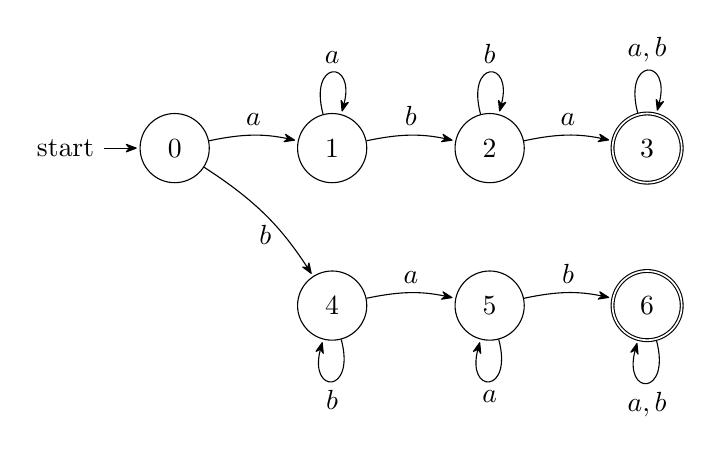
\begin{tikzpicture}[
    shorten >=1pt,          % Shortens arrows slightly so they don't touch node borders
    node distance=2.5cm,    % Sets global spacing between states
    on grid,                % Aligns positions based on center points instead of node borders
    auto,                   % Smart placement of transition labels
    >={Stealth[round]}      % Uses a clean, modern arrowhead style
]
\node[state, initial, initial where=left] (0) at (0,0)    {0};
\node[state]                              (1) at (2,0)    {1};
\node[state]                              (2) at (4,0)    {2};
\node[state, accepting]                   (3) at (6,0)    {3};
\node[state]                              (4) at (2,-2)    {4};
\node[state]                              (5) at (4,-2)    {5};
\node[state, accepting]                   (6) at (6,-2)    {6};

\path[->]
    (0) edge[bend left=12] node[above] {$a$} (1)
    (0) edge[bend left=12] node[below] {$b$} (4)
    (1) edge[bend left=12] node[above] {$b$} (2)
    (1) edge[loop above]    node        {$a$} (1)
    (2) edge[bend left=12] node[above] {$a$} (3)
    (2) edge[loop above]    node        {$b$} (2)
    (3) edge[loop above]    node        {$a,b$} (3)
    (4) edge[bend left=12] node[above] {$a$} (5)
    (4) edge[loop below]    node        {$b$} (4)
    (5) edge[bend left=12] node[above] {$b$} (6)
    (5) edge[loop below]    node        {$a$} (5)
    (6) edge[loop below]    node        {$a,b$} (6)
;
\end{tikzpicture}

\section*{Exercise 24}
The set of strings over \{\textit{a,b,c}\} that contain the substrings \textit{aa}, \textit{bb} and \textit{cc}.

\resizebox{\textwidth}{!}{
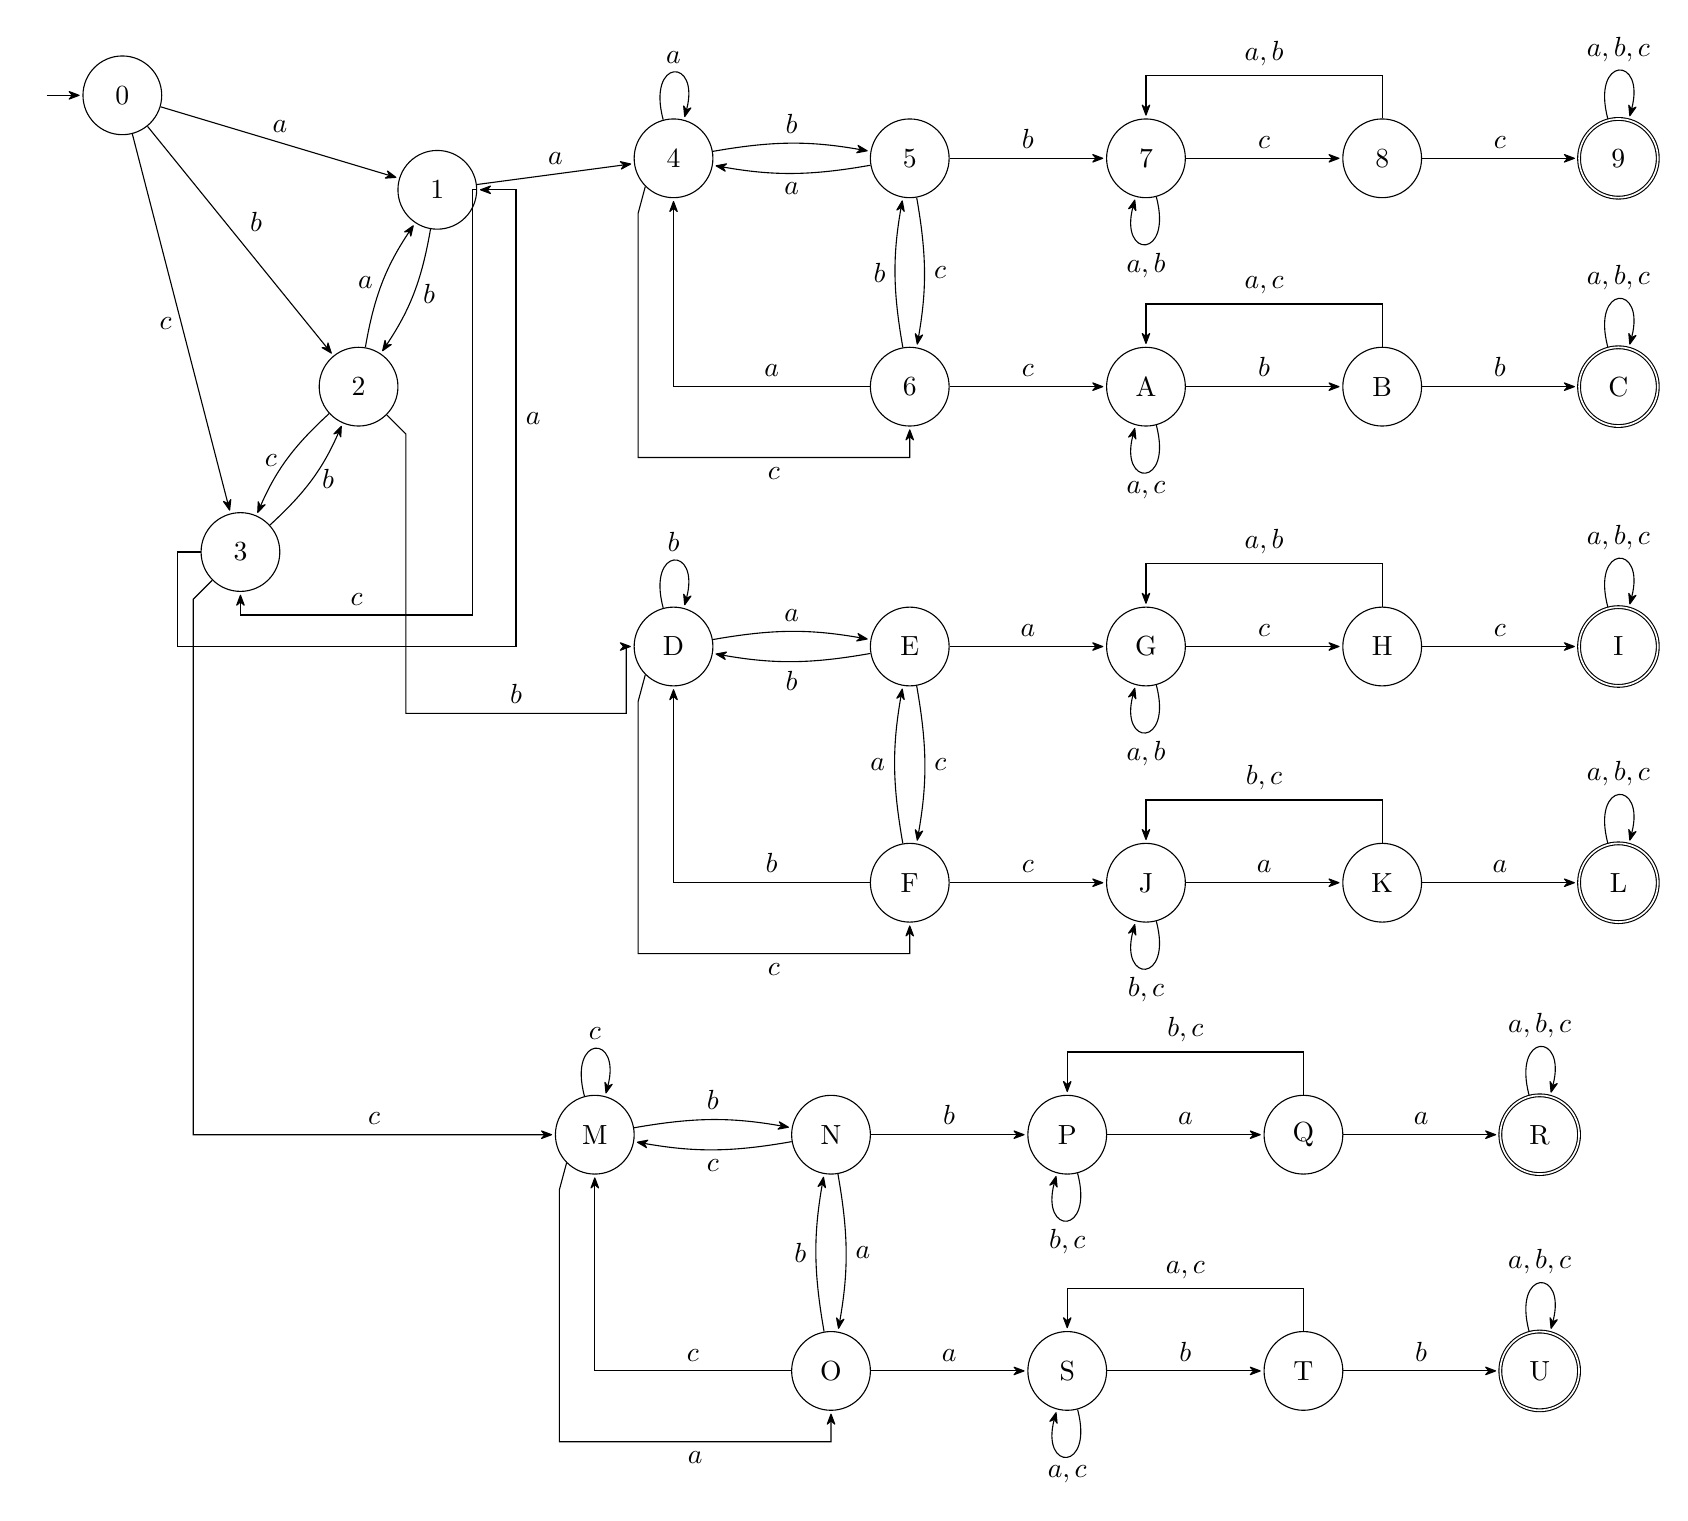
\begin{tikzpicture}[
    shorten >=1pt,          % Shortens arrows slightly so they don't touch node borders
    node distance=2.5cm,    % Sets global spacing between states
    on grid,                % Aligns positions based on center points instead of node borders
    auto,                   % Smart placement of transition labels
    >={Stealth[round]}      % Uses a clean, modern arrowhead style
]
\tikzset{
    every state/.style={minimum size=10mm},
    initial text={}
}

% Estados de entrada
\node[state, initial] (0) at (0,0)       {0};
\node[state]          (1) at (4,-1.2)    {1};
\node[state]          (2) at (3,-3.7)    {2};
\node[state]          (3) at (1.5,-5.8)  {3};

% Rama superior
\node[state]            (4) at (7,-0.8)   {4};
\node[state]            (5) at (10,-0.8)  {5};
\node[state]            (6) at (10,-3.7)  {6};

\node[state]            (7) at (13,-0.8)  {7};
\node[state]            (8) at (16,-0.8)  {8};
\node[state, accepting] (9) at (19,-0.8)  {9};

\node[state]            (A) at (13,-3.7)  {A};
\node[state]            (B) at (16,-3.7)  {B};
\node[state, accepting] (C) at (19,-3.7)  {C};

% Rama central
\node[state]            (D) at (7,-7)     {D};
\node[state]            (E) at (10,-7)    {E};
\node[state]            (F) at (10,-10)   {F};

\node[state]            (G) at (13,-7)    {G};
\node[state]            (H) at (16,-7)    {H};
\node[state, accepting] (I) at (19,-7)    {I};

\node[state]            (J) at (13,-10)   {J};
\node[state]            (K) at (16,-10)   {K};
\node[state, accepting] (L) at (19,-10)   {L};

% Rama inferior
\node[state]            (M) at (6,-13.2)  {M};
\node[state]            (N) at (9,-13.2)  {N};
\node[state]            (O) at (9,-16.2)  {O};

\node[state]            (P) at (12,-13.2) {P};
\node[state]            (Q) at (15,-13.2) {Q};
\node[state, accepting] (R) at (18,-13.2) {R};

\node[state]            (S) at (12,-16.2) {S};
\node[state]            (T) at (15,-16.2) {T};
\node[state, accepting] (U) at (18,-16.2) {U};

% Transiciones desde el estado inicial
\path[->]
    (0) edge node[above] {$a$} (1)
        edge node[above right] {$b$} (2)
        edge node[left] {$c$} (3);

% Transiciones entre 1, 2 y 3
\path[->]
    (1) edge[bend left=12] node[right] {$b$} (2)
    (2) edge[bend left=12] node[left]  {$a$} (1)
        edge[bend right=12] node[left] {$c$} (3)
    (3) edge[bend right=12] node[right] {$b$} (2);

% Caminos exteriores de 1 y 3
\draw[->]
    (1.east) -- (4.45,-1.2)
    -- (4.45,-6.6)
    -- node[above] {$c$} (1.5,-6.6)
    -- (3.south);

\draw[->]
    (3.west) -- (0.7,-5.8)
    -- (0.7,-7)
    -- (5,-7)
    -- node[right] {$a$} (5,-1.2)
    -- (1.east);

% Entrada a cada rama
\path[->]
    (1) edge node[above] {$a$} (4);

\draw[->]
    (2.south east) -- (3.6,-4.3)
    -- (3.6,-7.85)
    -- node[above] {$b$} (6.4,-7.85)
    -- (6.4,-7)
    -- (D.west);

\draw[->]
    (3.south west) -- (0.9,-6.4)
    -- (0.9,-13.2)
    -- node[above] {$c$} (M.west);

% Rama superior: estados 4, 5 y 6
\path[->]
    (4) edge[loop above] node {$a$} (4)
        edge[bend left=10] node[above] {$b$} (5)
    (5) edge[bend left=10] node[below] {$a$} (4)
        edge[bend left=10] node[right] {$c$} (6)
        edge node[above] {$b$} (7)
    (6) edge[bend left=10] node[left] {$b$} (5)
        edge node[above] {$c$} (A);

\draw[->]
    (4.south west) -- (6.55,-1.5)
    -- (6.55,-4.6)
    -- node[below] {$c$} (10,-4.6)
    -- (6.south);

\draw[->]
    (6.west) -- node[above] {$a$} (7,-3.7)
    -- (4.south);

% Rama superior: estados 7, 8 y 9
\path[->]
    (7) edge[loop below] node {$a,b$} (7)
        edge node[above] {$c$} (8)
    (8) edge node[above] {$c$} (9)
    (9) edge[loop above] node {$a,b,c$} (9);

\draw[->]
    (8.north) -- (16,0.25)
    -- node[above] {$a,b$} (13,0.25)
    -- (7.north);

% Rama superior: estados A, B y C
\path[->]
    (A) edge[loop below] node {$a,c$} (A)
        edge node[above] {$b$} (B)
    (B) edge node[above] {$b$} (C)
    (C) edge[loop above] node {$a,b,c$} (C);

\draw[->]
    (B.north) -- (16,-2.65)
    -- node[above] {$a,c$} (13,-2.65)
    -- (A.north);

% Rama central: estados D, E y F
\path[->]
    (D) edge[loop above] node {$b$} (D)
        edge[bend left=10] node[above] {$a$} (E)
    (E) edge[bend left=10] node[below] {$b$} (D)
        edge[bend left=10] node[right] {$c$} (F)
        edge node[above] {$a$} (G)
    (F) edge[bend left=10] node[left] {$a$} (E)
        edge node[above] {$c$} (J);

\draw[->]
    (D.south west) -- (6.55,-7.7)
    -- (6.55,-10.9)
    -- node[below] {$c$} (10,-10.9)
    -- (F.south);

\draw[->]
    (F.west) -- node[above] {$b$} (7,-10)
    -- (D.south);

% Rama central: estados G, H e I
\path[->]
    (G) edge[loop below] node {$a,b$} (G)
        edge node[above] {$c$} (H)
    (H) edge node[above] {$c$} (I)
    (I) edge[loop above] node {$a,b,c$} (I);

\draw[->]
    (H.north) -- (16,-5.95)
    -- node[above] {$a,b$} (13,-5.95)
    -- (G.north);

% Rama central: estados J, K y L
\path[->]
    (J) edge[loop below] node {$b,c$} (J)
        edge node[above] {$a$} (K)
    (K) edge node[above] {$a$} (L)
    (L) edge[loop above] node {$a,b,c$} (L);

\draw[->]
    (K.north) -- (16,-8.95)
    -- node[above] {$b,c$} (13,-8.95)
    -- (J.north);

% Rama inferior: estados M, N y O
\path[->]
    (M) edge[loop above] node {$c$} (M)
        edge[bend left=10] node[above] {$b$} (N)
    (N) edge[bend left=10] node[below] {$c$} (M)
        edge[bend left=10] node[right] {$a$} (O)
        edge node[above] {$b$} (P)
    (O) edge[bend left=10] node[left] {$b$} (N)
        edge node[above] {$a$} (S);

\draw[->]
    (M.south west) -- (5.55,-13.9)
    -- (5.55,-17.1)
    -- node[below] {$a$} (9,-17.1)
    -- (O.south);

\draw[->]
    (O.west) -- node[above] {$c$} (6,-16.2)
    -- (M.south);

% Rama inferior: estados P, Q y R
\path[->]
    (P) edge[loop below] node {$b,c$} (P)
        edge node[above] {$a$} (Q)
    (Q) edge node[above] {$a$} (R)
    (R) edge[loop above] node {$a,b,c$} (R);

\draw[->]
    (Q.north) -- (15,-12.15)
    -- node[above] {$b,c$} (12,-12.15)
    -- (P.north);

% Rama inferior: estados S, T y U
\path[->]
    (S) edge[loop below] node {$a,c$} (S)
        edge node[above] {$b$} (T)
    (T) edge node[above] {$b$} (U)
    (U) edge[loop above] node {$a,b,c$} (U);

\draw[->]
    (T.north) -- (15,-15.15)
    -- node[above] {$a,c$} (12,-15.15)
    -- (S.north);

\end{tikzpicture}
}

\section*{Exercise 25}
The set of strings over \{\textit{a,b,c}\} in which every \textit{b} is immediately followed by at least one \textit{c}.

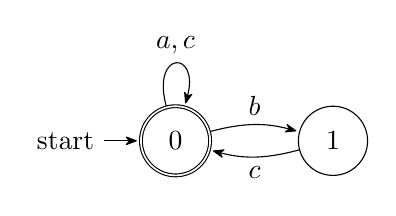
\begin{tikzpicture}[
    shorten >=1pt,          % Shortens arrows slightly so they don't touch node borders
    node distance=2.5cm,    % Sets global spacing between states
    on grid,                % Aligns positions based on center points instead of node borders
    auto,                   % Smart placement of transition labels
    >={Stealth[round]}      % Uses a clean, modern arrowhead style
]
\node[state, accepting, initial, initial where=left] (0) at (0,0){0};
\node[state]                              (1) at (2,0)    {1};

\path[->]
    (0) edge[bend left=15] node[above] {$b$} (1)
    (1) edge[bend left=15] node[below] {$c$} (0)
    (0) edge[loop above] node {$a,c$} (0)
;
\end{tikzpicture}

\section*{Exercise 26}
The set of strings over \{\textit{a,b,c}\} with length three.

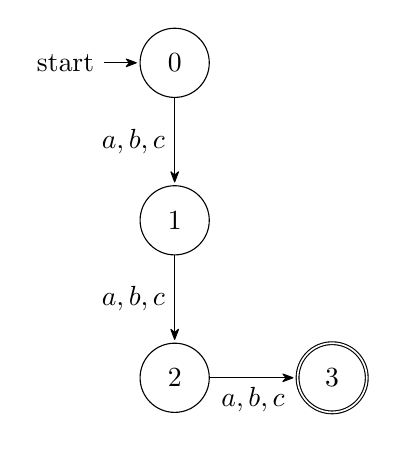
\begin{tikzpicture}[
    shorten >=1pt,          % Shortens arrows slightly so they don't touch node borders
    node distance=2.5cm,    % Sets global spacing between states
    on grid,                % Aligns positions based on center points instead of node borders
    auto,                   % Smart placement of transition labels
    >={Stealth[round]}      % Uses a clean, modern arrowhead style
]
\node[state, initial, initial where=left] (0) at (0,0)    {0};
\node[state]                              (1) at (0,-2)    {1};
\node[state]                              (2) at (0,-4)    {2};
\node[state, accepting]                   (3) at (2,-4)    {3};

\path[->]
    (0) edge node[left] {$a,b,c$} (1)
    (1) edge node[left] {$a,b,c$} (2)
    (2) edge node[below] {$a,b,c$} (3)

;
\end{tikzpicture}

\section*{Exercise 27}
The set of strings over \{\textit{a,b,c}\} with length less than three.

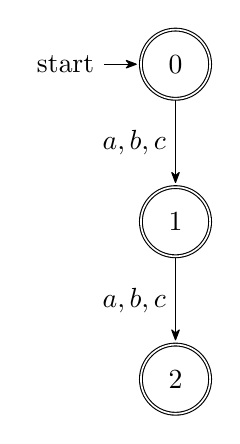
\begin{tikzpicture}[
    shorten >=1pt,          % Shortens arrows slightly so they don't touch node borders
    node distance=2.5cm,    % Sets global spacing between states
    on grid,                % Aligns positions based on center points instead of node borders
    auto,                   % Smart placement of transition labels
    >={Stealth[round]}      % Uses a clean, modern arrowhead style
]
\node[state, accepting, initial, initial where=left] (0) at (0,0)    {0};
\node[state, accepting]                              (1) at (0,-2)    {1};
\node[state, accepting]                              (2) at (0,-4)    {2};

\path[->]
    (0) edge node[left] {$a,b,c$} (1)
    (1) edge node[left] {$a,b,c$} (2)
;
\end{tikzpicture}

\section*{Exercise 28}
The set of strings over \{\textit{a,b,c}\} with length greater than three.

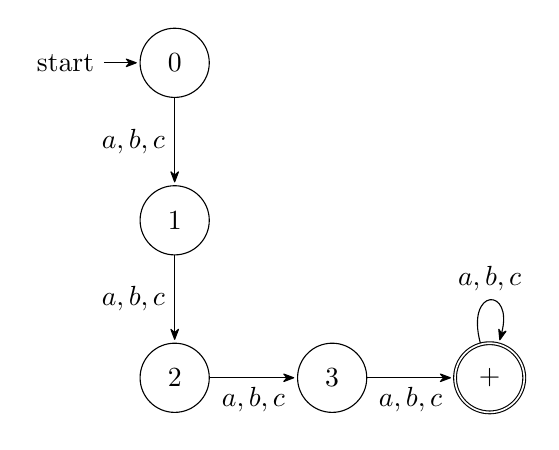
\begin{tikzpicture}[
    shorten >=1pt,          % Shortens arrows slightly so they don't touch node borders
    node distance=2.5cm,    % Sets global spacing between states
    on grid,                % Aligns positions based on center points instead of node borders
    auto,                   % Smart placement of transition labels
    >={Stealth[round]}      % Uses a clean, modern arrowhead style
]
\node[state, initial, initial where=left] (0) at (0,0)    {0};
\node[state]                              (1) at (0,-2)    {1};
\node[state]                              (2) at (0,-4)    {2};
\node[state]                              (3) at (2,-4)    {3};
\node[state,accepting]                    (+) at (4,-4)    {+};

\path[->]
    (0) edge node[left] {$a,b,c$} (1)
    (1) edge node[left] {$a,b,c$} (2)
    (2) edge node[below] {$a,b,c$} (3)
    (3) edge node[below] {$a,b,c$} (+)
    (+) edge[loop above] node {$a,b,c$} (+)
;
\end{tikzpicture}

\section*{Exercise 29}
The set of strings over \{\textit{a,b}\} in which the number of \textit{a}'s is divisible by three.

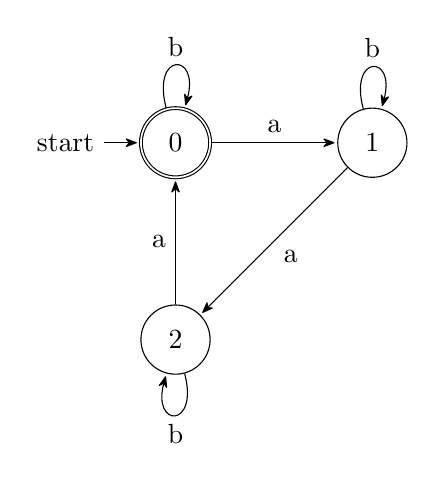
\begin{tikzpicture}[
    shorten >=1pt,          % Shortens arrows slightly so they don't touch node borders
    node distance=2.5cm,    % Sets global spacing between states
    on grid,                % Aligns positions based on center points instead of node borders
    auto,                   % Smart placement of transition labels
    >={Stealth[round]}      % Uses a clean, modern arrowhead style
]

    % --- 1. DEFINE THE STATES ---
    % Syntax: \node[<styles>] (<name>) [<relative position>] {<label>};
    \node[state, initial, accepting]    (0) {$0$};
    \node[state]                        (1) [right=of 0] {$1$};
    \node[state]                        (2) [below=of 0] {$2$};

    % --- 2. DEFINE THE TRANSITIONS ---
    \path[->] 
        (0) edge [loop above] node {b} ()
            edge node {a} (1)
        
        (1) edge [loop above] node {b} ()
            edge node {a} (2)
        
        (2) edge [loop below] node {b} ()
            edge node {a} (0);
\end{tikzpicture}

\newpage

\section*{Exercise 30}
The set of strings over \{\textit{a,b,c}\} in which the total number of \textit{b}'s and \textit{c}'s is three.

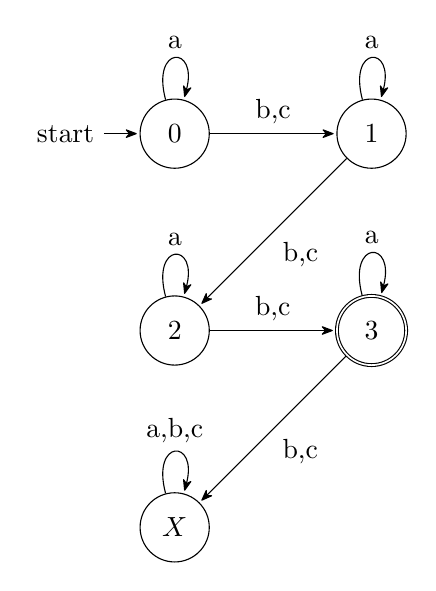
\begin{tikzpicture}[
    shorten >=1pt,          % Shortens arrows slightly so they don't touch node borders
    node distance=2.5cm,    % Sets global spacing between states
    on grid,                % Aligns positions based on center points instead of node borders
    auto,                   % Smart placement of transition labels
    >={Stealth[round]}      % Uses a clean, modern arrowhead style
]

    % --- 1. DEFINE THE STATES ---
    % Syntax: \node[<styles>] (<name>) [<relative position>] {<label>};
    \node[state, initial]       (0) {$0$};
    \node[state]                (1) [right=of 0] {$1$};
    \node[state]                (2) [below=of 0] {$2$};
    \node[state, accepting]     (3) [right=of 2] {$3$};
    \node[state]                (X) [below=of 2] {$X$};

    % --- 2. DEFINE THE TRANSITIONS ---
    \path[->] 
        (0) edge [loop above] node {a} ()
            edge node {b,c} (1)
        
        (1) edge [loop above] node {a} ()
            edge node {b,c} (2)
        
        (2) edge [loop above] node {a} ()
            edge node {b,c} (3)

        (3) edge [loop above] node {a} ()
            edge node {b,c} (X)

        (X) edge [loop above] node {a,b,c} ();
\end{tikzpicture}

\section*{Exercise 31}
The set of strings over \{\textit{a,b}\} in which every \textit{a} is either immediately preceded o immediately followed by \textit{b}, for example, \textit{baab}, \textit{aba}, and \textit{b}.

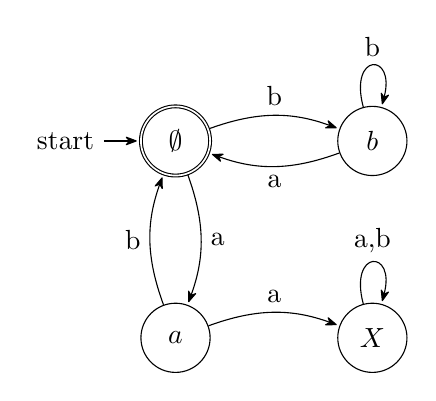
\begin{tikzpicture}[
    shorten >=1pt,          % Shortens arrows slightly so they don't touch node borders
    node distance=2.5cm,    % Sets global spacing between states
    on grid,                % Aligns positions based on center points instead of node borders
    auto,                   % Smart placement of transition labels
    >={Stealth[round]}      % Uses a clean, modern arrowhead style
]

    % --- 1. DEFINE THE STATES ---
    % Syntax: \node[<styles>] (<name>) [<relative position>] {<label>};
    \node[state, initial, accepting]        (0) {$\emptyset$};
    \node[state]                            (a) [below=of 0] {$a$};
    \node[state]                            (b) [right=of 0] {$b$};
    \node[state]                            (X) [right=of a] {$X$};

    % --- 2. DEFINE THE TRANSITIONS ---
    \path[->] 
        (0) edge [bend left=20] node {a} (a)
            edge [bend left=20] node {b} (b)
        
        (a) edge [bend left=20] node {a} (X)
            edge [bend left=20] node {b} (0)
        
        (b) edge [loop above] node {b} ()
            edge [bend left=20] node {a} (0)

        (X) edge [loop above] node {a,b} ();
\end{tikzpicture}

\newpage

\section*{Exercise 32}
The set of strings of odd length over \{\textit{a,b}\} that contain the substring \textit{bb}.

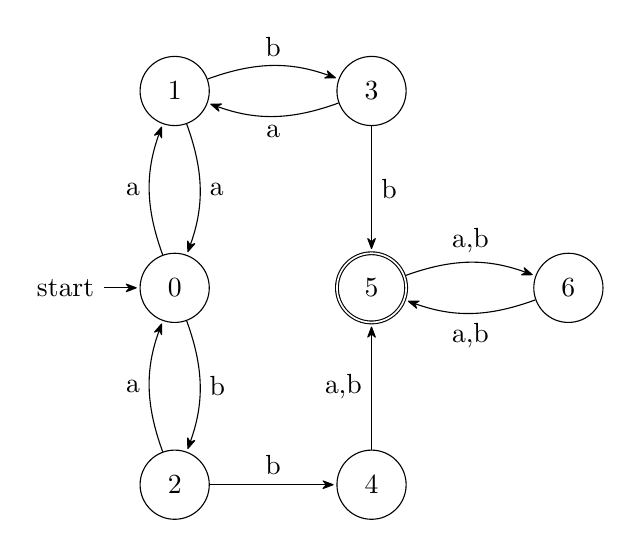
\begin{tikzpicture}[
    shorten >=1pt,          % Shortens arrows slightly so they don't touch node borders
    node distance=2.5cm,    % Sets global spacing between states
    on grid,                % Aligns positions based on center points instead of node borders
    auto,                   % Smart placement of transition labels
    >={Stealth[round]}      % Uses a clean, modern arrowhead style
]

    % --- 1. DEFINE THE STATES ---
    % Syntax: \node[<styles>] (<name>) [<relative position>] {<label>};
    \node[state, initial]   (0) {$0$};
    \node[state]            (1) [above=of 0] {$1$};
    \node[state]            (2) [below=of 0] {$2$};
    \node[state]            (3) [right=of 1] {$3$};
    \node[state]            (4) [right=of 2] {$4$};
    \node[state, accepting] (5) [below=of 3] {$5$};
    \node[state]            (6) [right=of 5] {$6$};

    % --- 2. DEFINE THE TRANSITIONS ---
    \path[->] 
        (0) edge [bend left=20] node {a} (1)
            edge [bend left=20] node {b} (2)
        
        (1) edge [bend left=20] node {b} (3)
            edge [bend left=20] node {a} (0)
        
        (2) edge [bend left=20] node {a} (0)
            edge node {b} (4)

        (3) edge [bend left=20] node {a} (1)
            edge node {b} (5)

        (4) edge node {a,b} (5)

        (5) edge [bend left=20] node {a,b} (6)

        (6) edge [bend left=20] node {a,b} (5);
\end{tikzpicture}

\section*{Exercise 33}
The set of strings of even length over \{\textit{a,b,c}\} that contain exactly one \textit{a}.

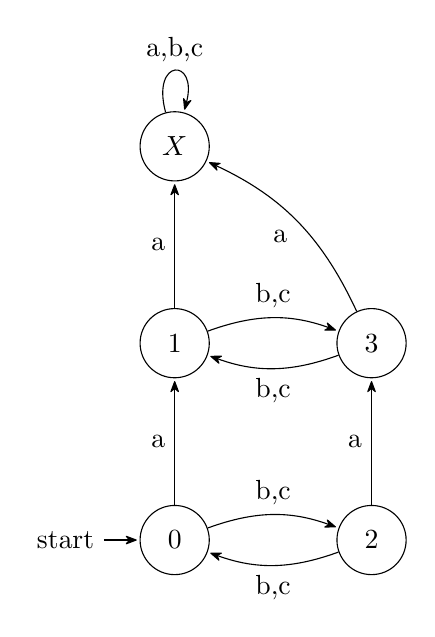
\begin{tikzpicture}[
    shorten >=1pt,          % Shortens arrows slightly so they don't touch node borders
    node distance=2.5cm,    % Sets global spacing between states
    on grid,                % Aligns positions based on center points instead of node borders
    auto,                   % Smart placement of transition labels
    >={Stealth[round]}      % Uses a clean, modern arrowhead style
]

    % --- 1. DEFINE THE STATES ---
    % Syntax: \node[<styles>] (<name>) [<relative position>] {<label>};
    \node[state, initial]   (0) {$0$};
    \node[state]            (1) [above=of 0] {$1$};
    \node[state]            (2) [right=of 0] {$2$};
    \node[state]            (3) [above=of 2] {$3$};
    \node[state]            (X) [above=of 1] {$X$};

    % --- 2. DEFINE THE TRANSITIONS ---
    \path[->] 
        (0) edge node {a} (1)
            edge [bend left=20] node {b,c} (2)
        
        (1) edge node {a} (X)
            edge [bend left=20] node {b,c} (3)
        
        (2) edge node {a} (3)
            edge [bend left=20] node {b,c} (0)

        (3) edge [bend right=20] node {a} (X)
            edge [bend left=20] node {b,c} (1)

        (X) edge [loop above] node {a,b,c} ();
\end{tikzpicture}

\newpage

\section*{Exercise 34}
The set of strings over \{\textit{a,b,c}\} with an odd number of occurrences of the substring \textit{ab}.

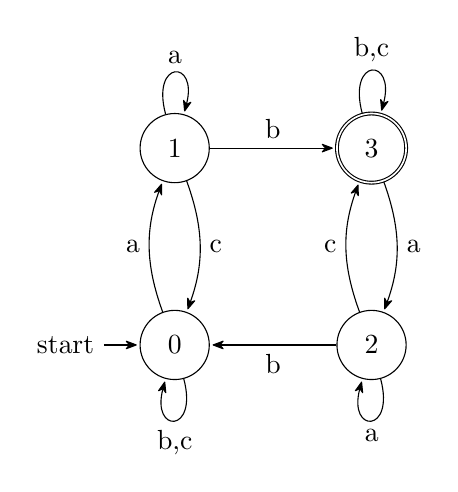
\begin{tikzpicture}[
    shorten >=1pt,          % Shortens arrows slightly so they don't touch node borders
    node distance=2.5cm,    % Sets global spacing between states
    on grid,                % Aligns positions based on center points instead of node borders
    auto,                   % Smart placement of transition labels
    >={Stealth[round]}      % Uses a clean, modern arrowhead style
]

    % --- 1. DEFINE THE STATES ---
    % Syntax: \node[<styles>] (<name>) [<relative position>] {<label>};
    \node[state, initial]   (0) {$0$};
    \node[state]            (1) [above=of 0] {$1$};
    \node[state]            (2) [right=of 0] {$2$};
    \node[state, accepting] (3) [above=of 2] {$3$};

    % --- 2. DEFINE THE TRANSITIONS ---
    \path[->] 
        (0) edge [loop below] node {b,c} ()
            edge [bend left=20] node {a} (1)
        
        (1) edge [loop above] node {a} ()
            edge node {b} (3)
            edge [bend left=20] node {c} (0)
        
        (2) edge [loop below] node {a} ()
            edge node {b} (0)
            edge [bend left=20] node {c} (3)

        (3) edge [loop above] node {b,c} ()
            edge [bend left=20] node {a} (2);
\end{tikzpicture}

\section*{Exercise 35}
The set of strings of odd length over \{\textit{a,b}\} that contain exactly two \textit{b}'s.

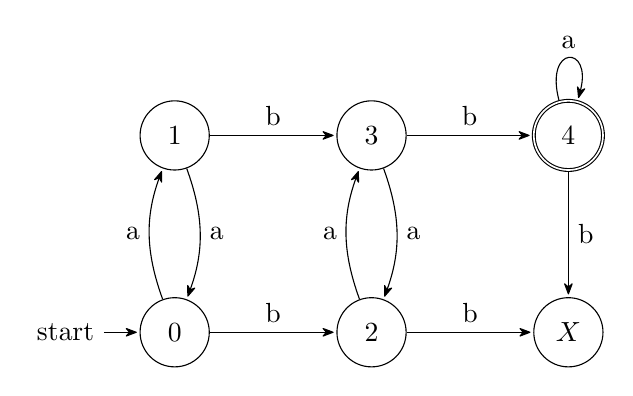
\begin{tikzpicture}[
    shorten >=1pt,          % Shortens arrows slightly so they don't touch node borders
    node distance=2.5cm,    % Sets global spacing between states
    on grid,                % Aligns positions based on center points instead of node borders
    auto,                   % Smart placement of transition labels
    >={Stealth[round]}      % Uses a clean, modern arrowhead style
]

    % --- 1. DEFINE THE STATES ---
    % Syntax: \node[<styles>] (<name>) [<relative position>] {<label>};
    \node[state, initial]   (0) {$0$};
    \node[state]            (1) [above=of 0] {$1$};
    \node[state]            (2) [right=of 0] {$2$};
    \node[state]            (3) [above=of 2] {$3$};
    \node[state, accepting] (4) [right=of 3] {$4$};
    \node[state]            (X) [right=of 2] {$X$};

    % --- 2. DEFINE THE TRANSITIONS ---
    \path[->] 
        (0) edge [bend left=20] node {a} (1)
            edge node {b} (2)
        
        (1) edge [bend left=20] node {a} (0)
            edge node {b} (3)
        
        (2) edge [bend left=20] node {a} (3)
            edge node {b} (X)

        (3) edge [bend left=20] node {a} (2)
            edge node {b} (4)

        (4) edge [loop above] node {a} ()
            edge node {b} (X);
\end{tikzpicture}

\newpage

\section*{Exercise 36}
The set of strings over \{\textit{a,b}\} with an even number of \textit{a}'s or an odd number of \textit{b}'s.

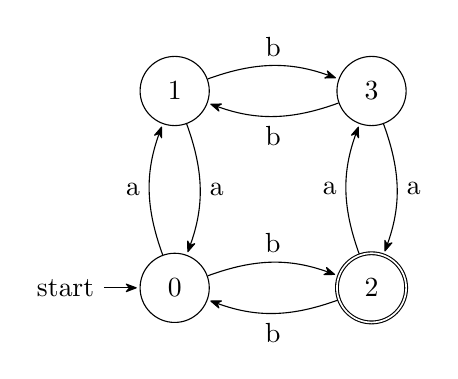
\begin{tikzpicture}[
    shorten >=1pt,          % Shortens arrows slightly so they don't touch node borders
    node distance=2.5cm,    % Sets global spacing between states
    on grid,                % Aligns positions based on center points instead of node borders
    auto,                   % Smart placement of transition labels
    >={Stealth[round]}      % Uses a clean, modern arrowhead style
]

    % --- 1. DEFINE THE STATES ---
    % Syntax: \node[<styles>] (<name>) [<relative position>] {<label>};
    \node[state, initial]   (0) {$0$};
    \node[state]            (1) [above=of 0] {$1$};
    \node[state, accepting] (2) [right=of 0] {$2$};
    \node[state]            (3) [above=of 2] {$3$};

    % --- 2. DEFINE THE TRANSITIONS ---
    \path[->] 
        (0) edge [bend left=20] node {a} (1)
            edge [bend left=20] node {b} (2)
        
        (1) edge [bend left=20] node {a} (0)
            edge [bend left=20] node {b} (3)
        
        (2) edge [bend left=20] node {a} (3)
            edge [bend left=20] node {b} (0)

        (3) edge [bend left=20] node {a} (2)
            edge [bend left=20] node {b} (1);
\end{tikzpicture}

\end{document}
